One of the defining properties of topological insulators is the presence of conducting edge states with an insulating bulk. The example considered here in sec. \ref{sec:ti_exemples} is a two dimensionnal material and its edge is therefore one-dimensionnal. The QH and QSH effects both involve one-dimensionnal conduction. In one dimension, electrons can only either move forward of backward on the edge of the sample and this restriction is central for Hall effects. \cite{qi_quantum_2010}.  
\subsection{QH}
\begin{figure}[h!]
    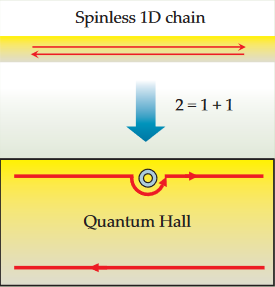
\includegraphics[scale = 0.7]{sections/visuel/spinless.png}
    \caption{Schematic representation of the conduction chanels in a spinless quantum Hall system.\cite{qi_quantum_2010}}
    \label{spinless}
\end{figure}

\subsubsection{Chern number}

The chern number is a topological invariant closely related to the Euler characteristic.

\subsubsection{Impossiblity of backscattering}

\subsubsection{In which material does it happen}

\subsection{QSH}

\begin{figure}[h!]
    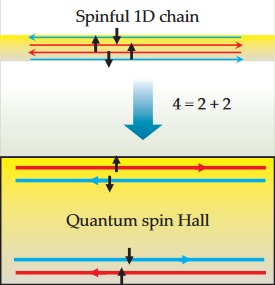
\includegraphics[scale = 0.7]{sections/visuel/spinful.png}
    \caption{Schematic representation of the conduction chanels in a spinlful quantum Hall system.}
    \label{spinful}
\end{figure}

% Talk about the fact that the states are topologicaly protected since their edge states survive the addition of impurities \cite{kane_this_2011}